\section{Условие задания}

Содержание проекта: Команда разработчиков из 16 человек занимается созданием карты города на основе собственного модуля отображения. Проект должен быть завершен в течение 6 месяцев. Бюджет проекта: 50 000 рублей.

\section{Задача 1}

Выведем таблицу освоенного объема.

\begin{figure}[H]
    \centering
    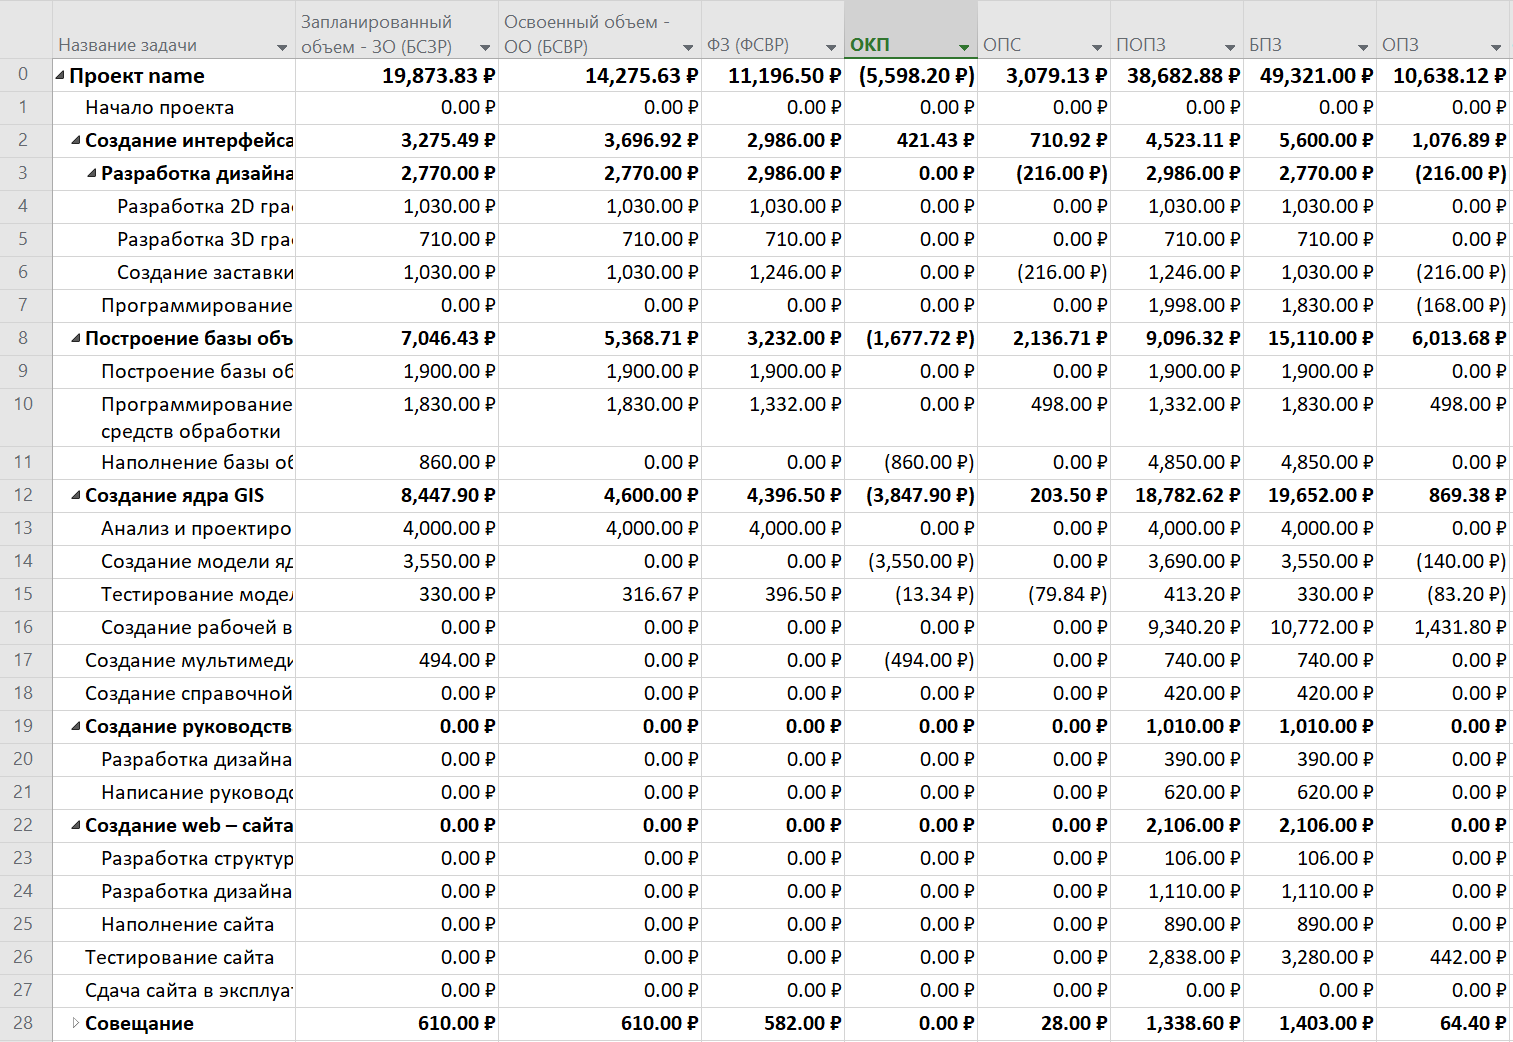
\includegraphics[width=0.8\textwidth]{img/content/task_01.png}
    \caption{Таблица освоенного объема}
    \label{fig:task_01}
\end{figure}

\textbf{Запланированный объем} (ЗО) -- средства, которые были бы затрачены на выполнение с начала проекта до выбранной даты отчета, если бы задача точно соответствовала графику и смете. В случае нашего проекта: 19 873.83 рубля.

\textbf{Базовая стоимость выполненных работ} (БСВР) -- средства, которые были бы затрачены на выполнение задачи с самого начала проекта до выбранной даты отчета, если бы фактически выполненная работа оплачивалась согласно смете. В случае проекта: 14 275.63 рубля (отклонение от базовой стоимости запланированных работ -- 5 598.20 рублей).

\textbf{Фактические затраты или фактическая стоимость выполненных работ} (ФСВР) -- средства, фактически потраченные на выполнение задачи в период с начала проекта до выбранной даты отчета. В случае проекта: 11 196.50 рублей (отклонение от базовой стоимости выполненных работ 2 079.13 рублей). 

\textbf{Предварительная оценка по завершении} (ПОПЗ) -- отображает ожидаемые общие затраты, расчет которых основан на предположении, что оставшаяся часть работы будет выполнена в точном соответствии со сметой. Для проекта: 38 682.88 рубля.

\section{Задача 2}

Исходя из отчета о бюджетной стоимости можно сказать, что аибольшие затраты пришлись на 28 неделю. В это время выполнялись следующие задачи

\begin{itemize}
    \item Программирование интерфейса
    \item Наполнение базы объектов
    \item Разработка дизайна руководства
    \item Написание руководства пользователя
    \item Разработка структуры сайта
    \item Разработка дизайна сайта
\end{itemize}

\begin{figure}[H]
    \centering
    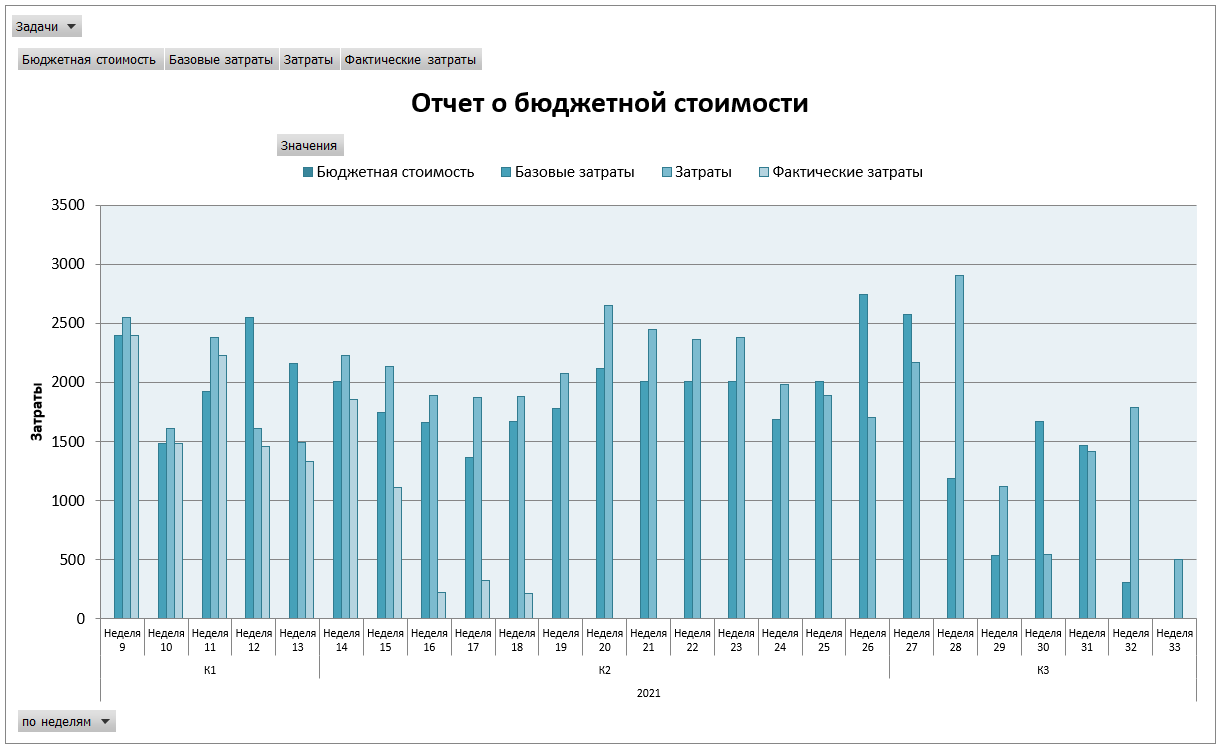
\includegraphics[width=0.8\textwidth]{img/content/task_02_1.png}
    \caption{Отчет о бюджетной стоимости}
    \label{fig:task_02_1}
\end{figure}

Исходи из превышения затрат на задачи можно заметить, что задачи создание интерфейса, построение базы объектов, создание ядра GIS и тестирование сайта превышают базовые затраты.

\begin{figure}[H]
    \centering
    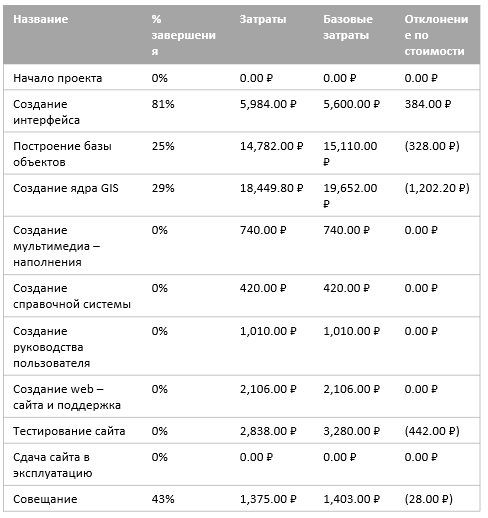
\includegraphics[width=0.8\textwidth]{img/content/task_02_2.png}
    \caption{Превышение затрат на задачи}
    \label{fig:task_02_2}
\end{figure}

\section{Задача 3}

Далее была разработана новая декомпозиция задач.

\begin{figure}[H]
    \centering
    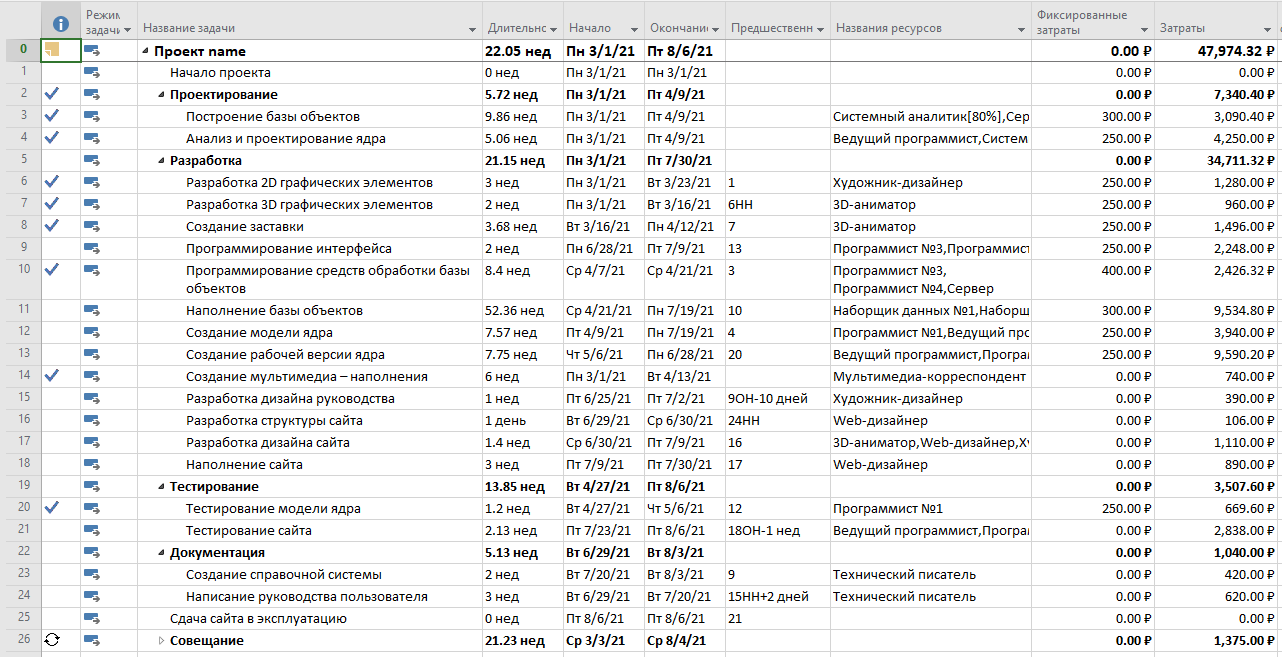
\includegraphics[width=0.8\textwidth]{img/content/task_03.png}
    \caption{Декомпозиция}
    \label{fig:task_03}
\end{figure}

В результате декомпозиции окончание сместилось до 8 августа, а бюджет упал до 47 974 рублей.

\section{Выводы}


В проекте был проведен анализ базового и фактического плана на 5 мая 2021.

У руководителя проекта наибольшая потребность в средствах возникнет на 28 неделе. Проведен альтернативный вариант декомпозиции задачи, в ходе которой время выполнения проекта уменьшилась на 10 дней, а бюджет уменьшился на 636 рублей.
